\begin{figure*}[ht]
  
  \begin{subfigure}{.315\textwidth}
    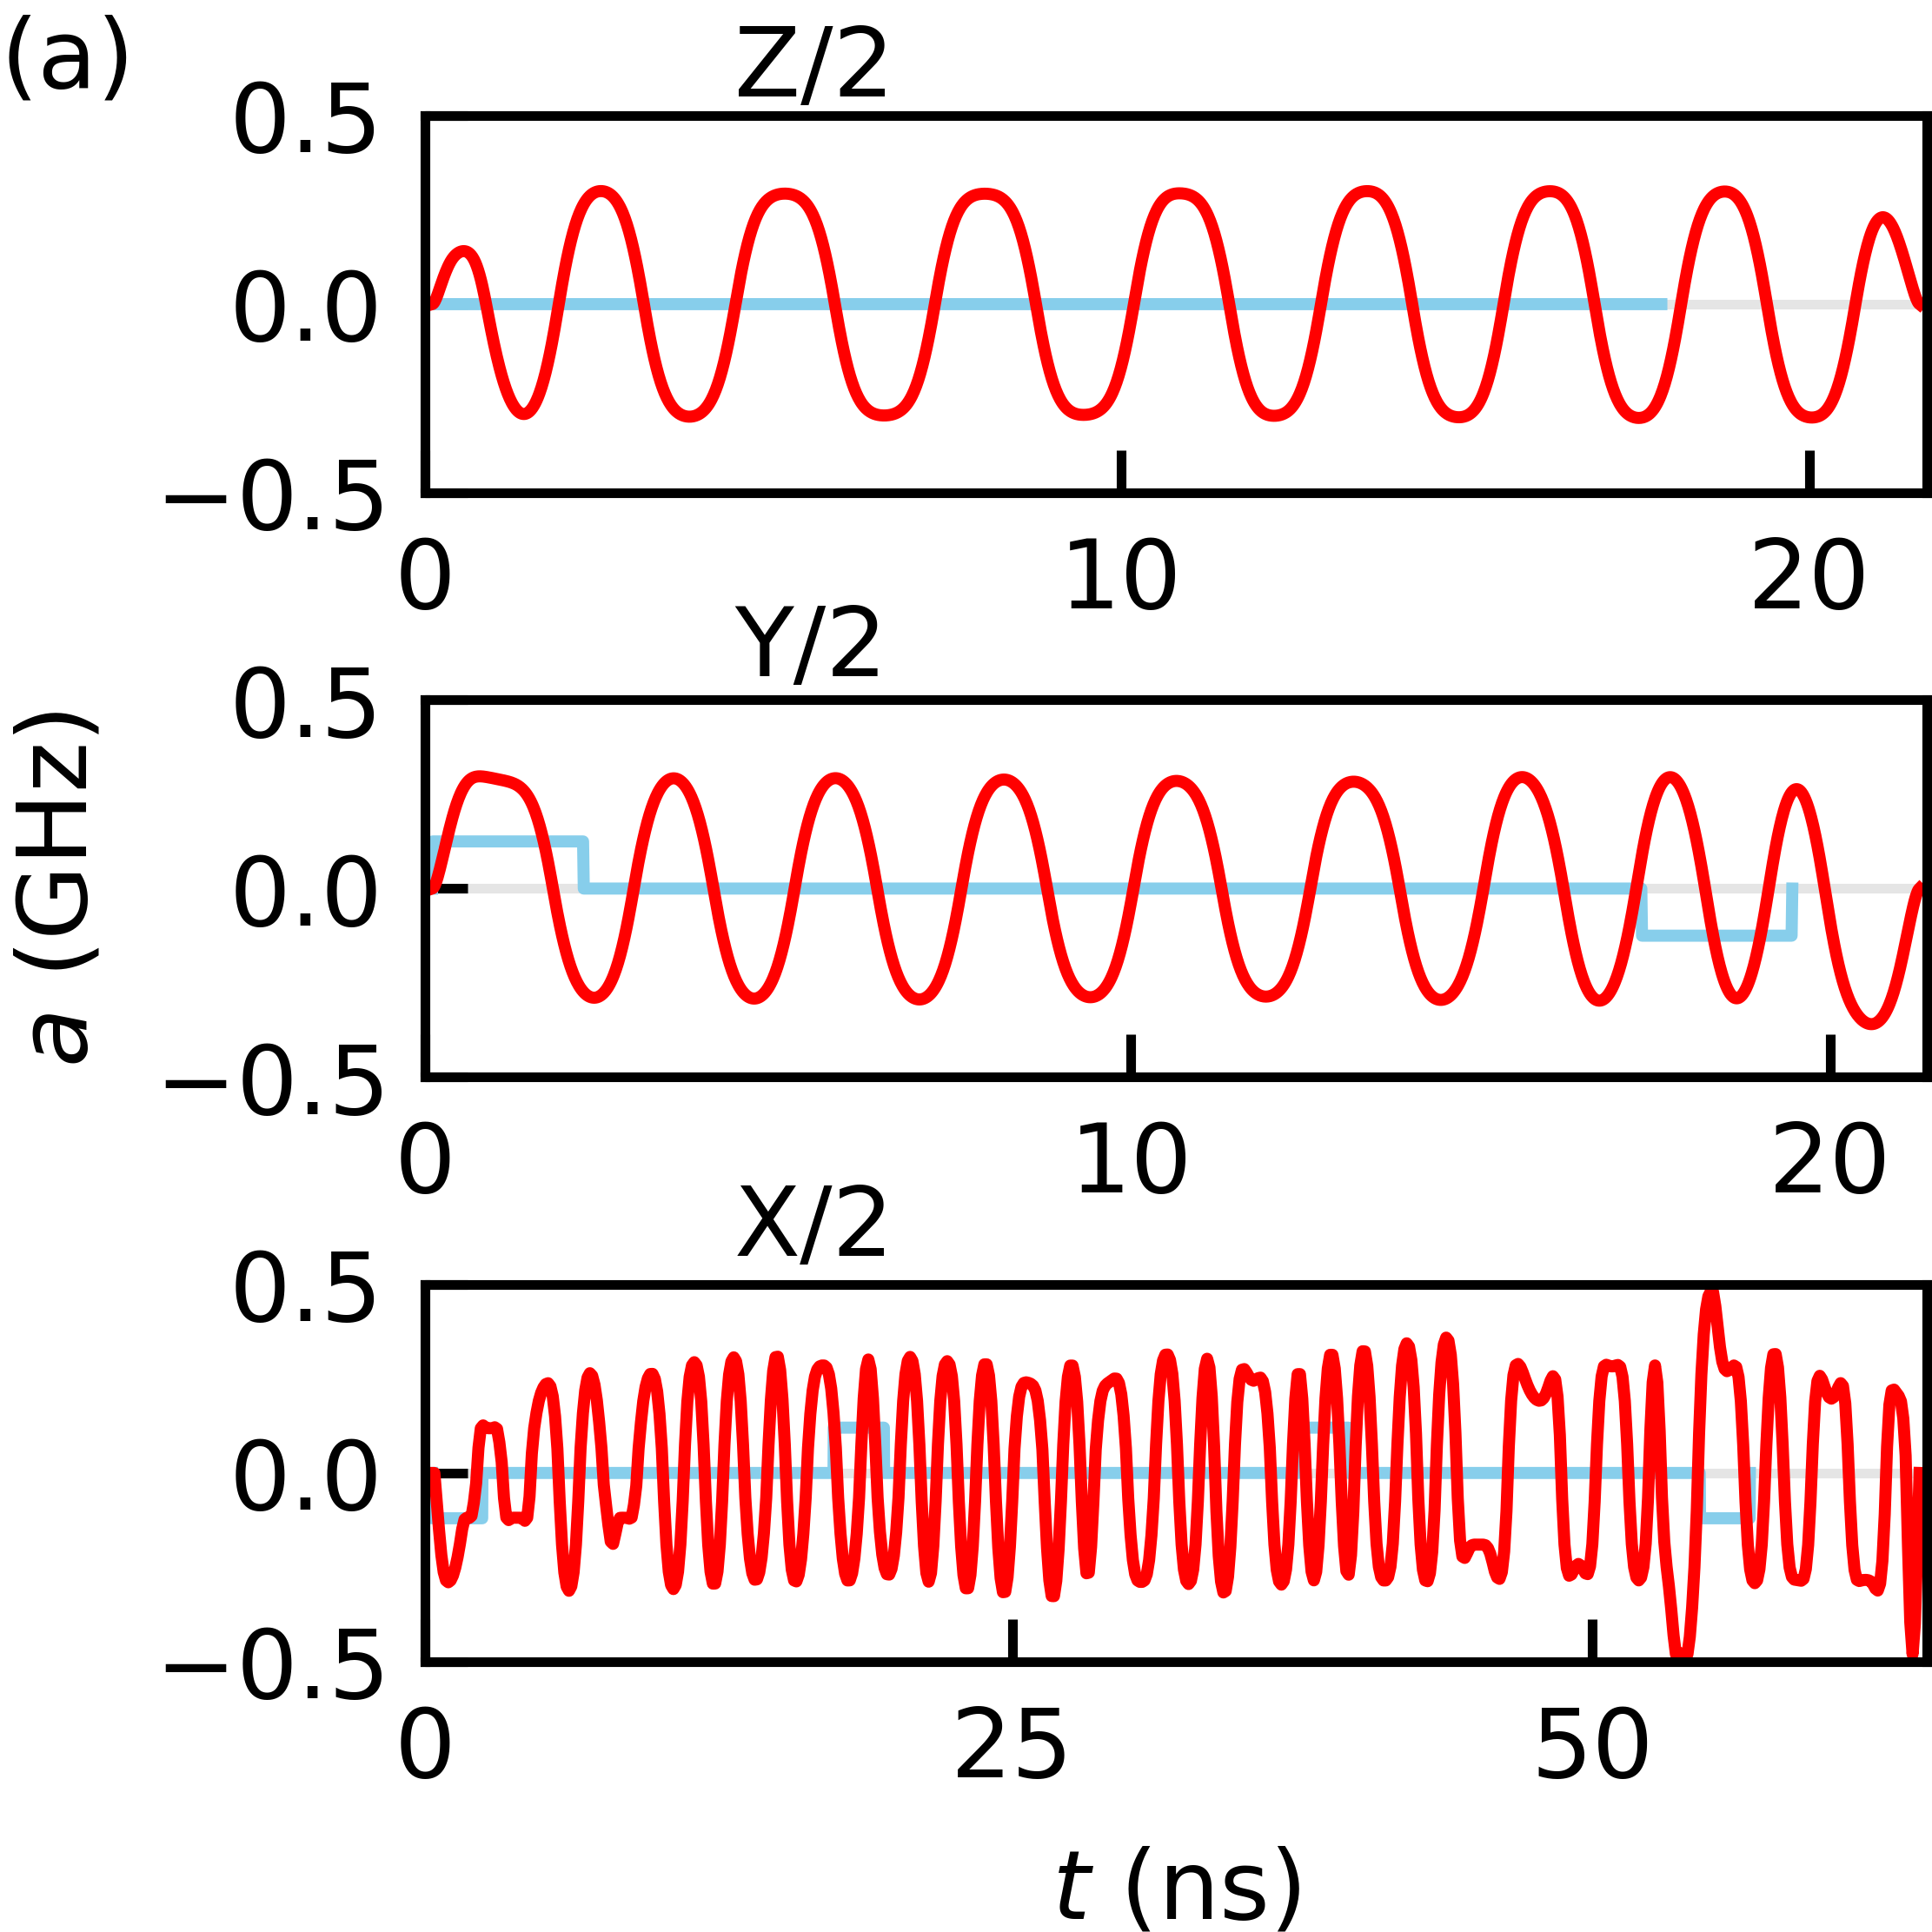
\includegraphics[width=\linewidth]{assets/f1a.png}
    \caption{\label{fig:longitudea}}
  \end{subfigure}\hfill
  \begin{subfigure}{.23\textwidth}
    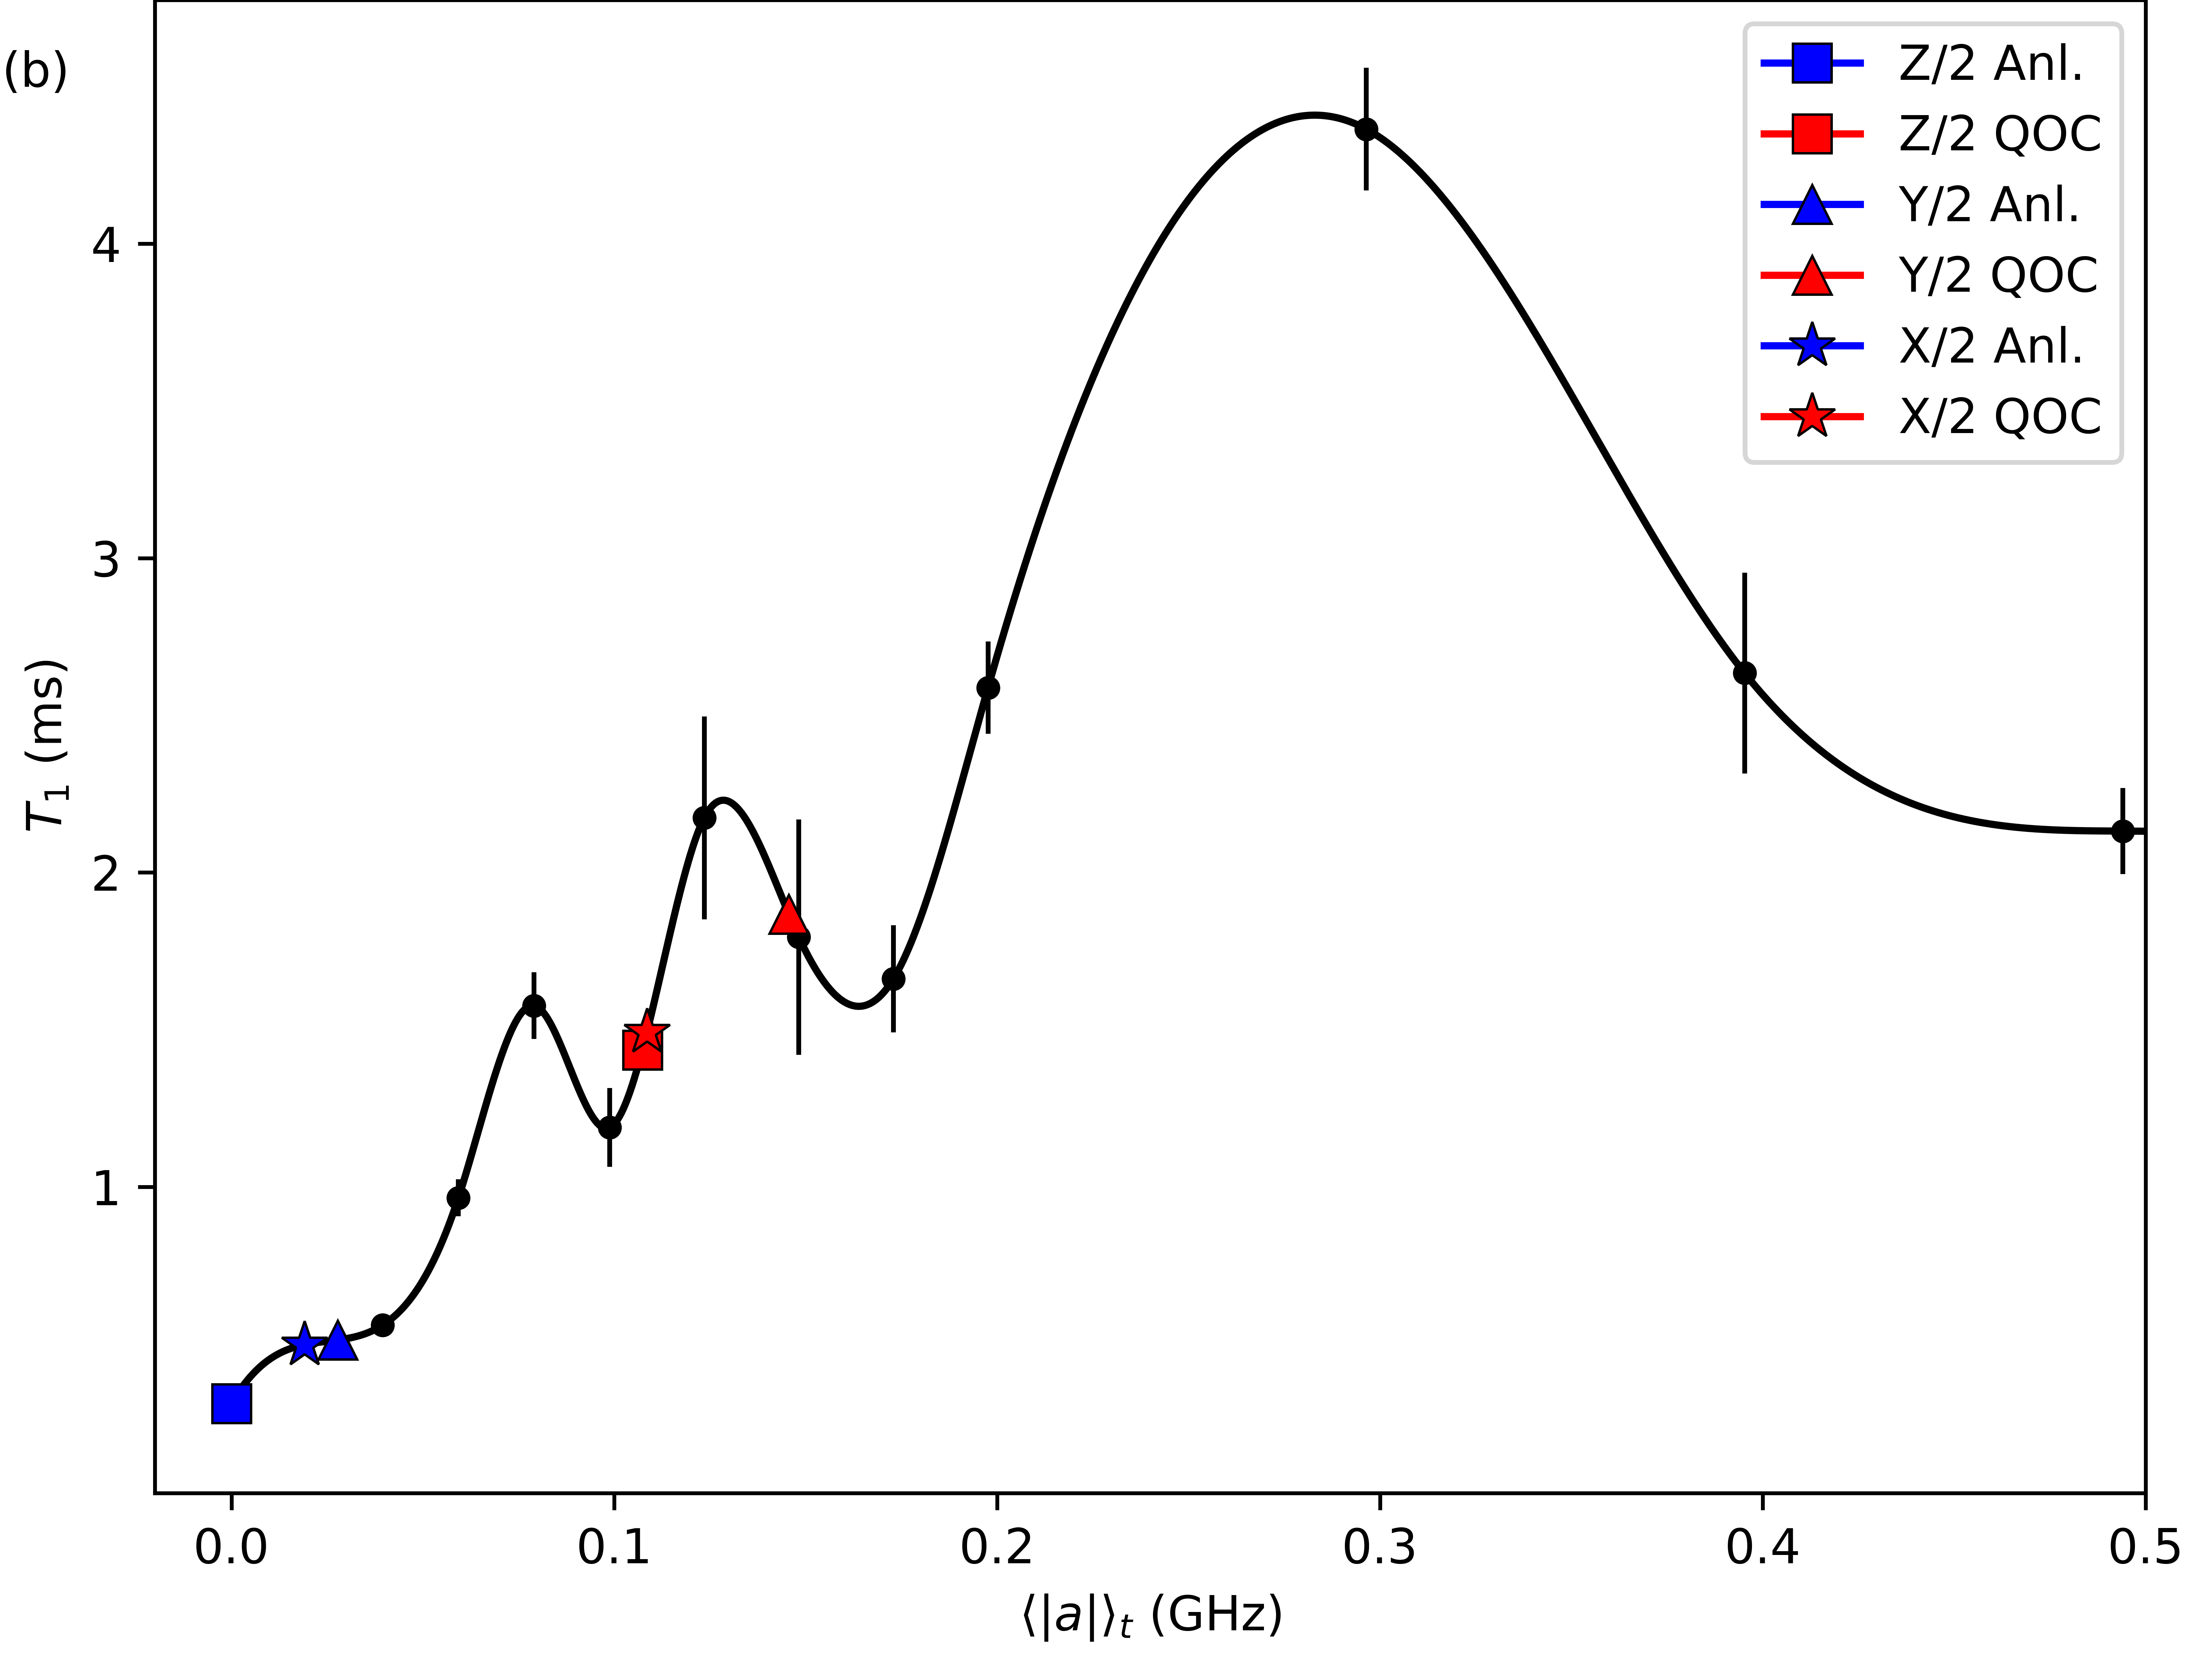
\includegraphics[width=\linewidth]{assets/f1b.png}
    \caption{\label{fig:longitudeb}}
  \end{subfigure}\hfill
  \begin{subfigure}{.4\textwidth}
    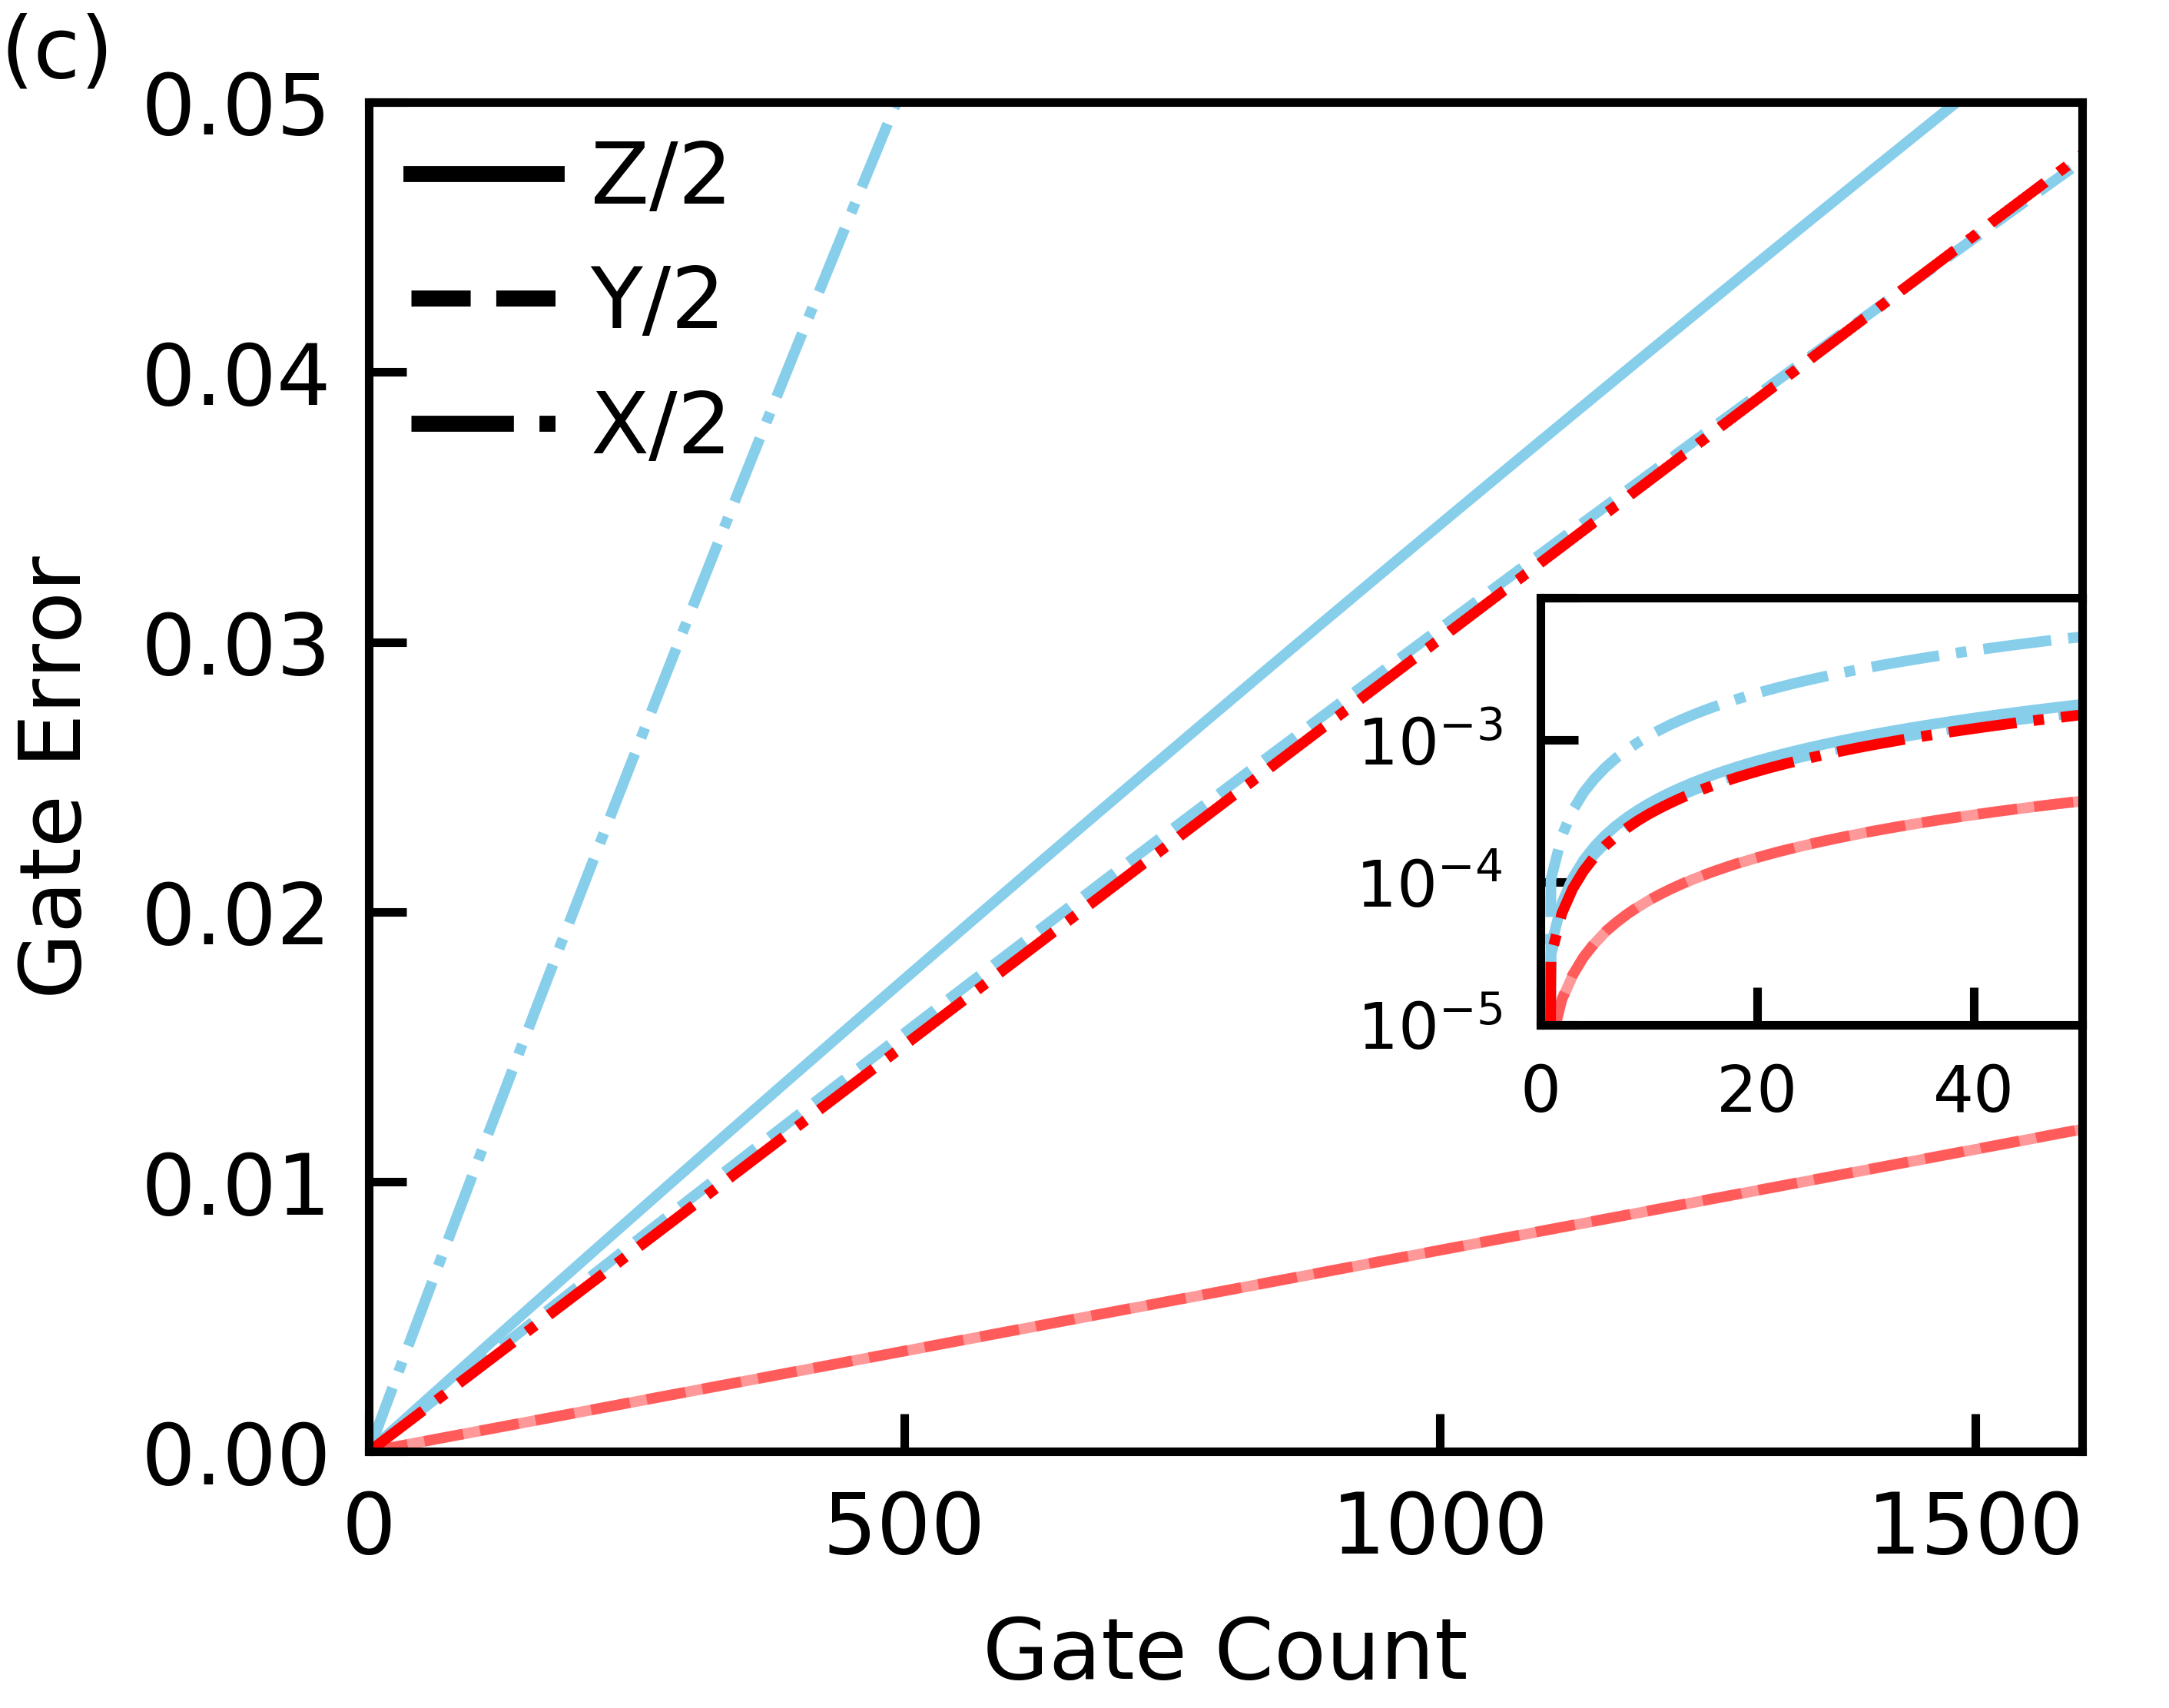
\includegraphics[width=\linewidth]{assets/f1c.png}
    \caption{\label{fig:longitudec}}
  \end{subfigure}
  \caption{
    (a) Numerically optimized gates (red) and analytically optimized gates (blue).
    (b) $T_{1}$ interpolation function used in optimization. Markers
    denote the time-averaged, absolute amplitude of each gate.
    (c) Lindblad master equation simulation with $T_{1}$ dissipation
    for successive gate applications. The cumulative
    gate error is computed after each gate application.
    The numerically optimized $Z/2$ and $Y/2$ gate errors are indistinguishable.
  }
  \label{fig:longitude}
\end{figure*}

\section{Longitudinal Relaxation Awareness \label{sec:longitude}}
The strength of longitudinal relaxation type decoherence varies
with the control parameters in a range of superconducting circuit platforms,
including the fluxonium qubit. Because dissipation to the thermal bath
via longitudinal relaxation is an irreversible process that results in information loss,
it is advantageous to tune the controls to extend the longitudinal
relaxation time $T_{1}$--which represents the $1/e$ decay time
of the quantum state.
Computing the gate error due to longitudinal relaxation
requires propagating density matrices of size $n \times n$ under master equation
dynamics, rather than state vectors of size $n$ under the TDSE dynamics \eqref{eq:tdse}.
We avoid this increase in computational complexity by
penalizing the probability (integrated rate) of longitudinal relaxation.
Using this probability as proxy for the gate error incurred
is reasonable because losses due to longitudinal relaxation increase monotonically
in time.
This technique can be extended to
error channels which share the monotonically increasing property.
Additionally, for a constant $T_{1}$ time, a shorter gate duration
would favor a lower longitudinal relaxation probability. We allow
the optimizer to tune the gate duration in order to minimize the
longitudinal relaxation probability. Our scheme for time-optimal
control is applicable to any time-optimal problem, not only
the one we study here.

The longitudinal relaxation probability is given by,
\begin{equation}
  P_{1}(t) = \int_{0}^{t} T_{1}^{-1}(a(t^{\prime})) dt^{\prime}
\end{equation}
This value is appended to the augmented state vector \eqref{eq:astatecontrols}
and penalized according to \eqref{eq:costfun}.
$T_{1}(a_{k})$ is obtained at each knot point by evaluating
a spline fit to experimental data of the form $\{(a, T_{1})\}$,
see Figure \ref{fig:longitudeb}.
It is also possible to fit a spline to theoretically obtained data.
However, $T_{1}$ values are known to fluctuate greatly
with laboratory temperatures \cite{klimov2018fluctuations}.
Interpolating $T_{1}$ from experimental data
increases the fridge truth of the simulation.

We allow the optimizer to tune the gate duration by
making the time step between each knot point $\Delta t_{k}$
a decision variable. Promoting $\Delta t_{k}$ to a decision variable, rather
than the number of knot points $N$, preserves the
Markovian decision structure of the trajectory
optimization problem. The square root of the time step $\sqrt{\Delta t_{k}}$
is appended to the augmented control vector \eqref{eq:astatecontrols}
and the squared root
of the time step $\lvert \Delta t_{k} \rvert$ is used
for integration in the discrete dynamics function \eqref{eq:dyn_con}.
To ensure numerical
integration accuracy is maintained we add a bound
constraint on the time step at each knot point.

%% F2
\begin{figure*}[ht]
  \begin{subfigure}{.315\textwidth}
    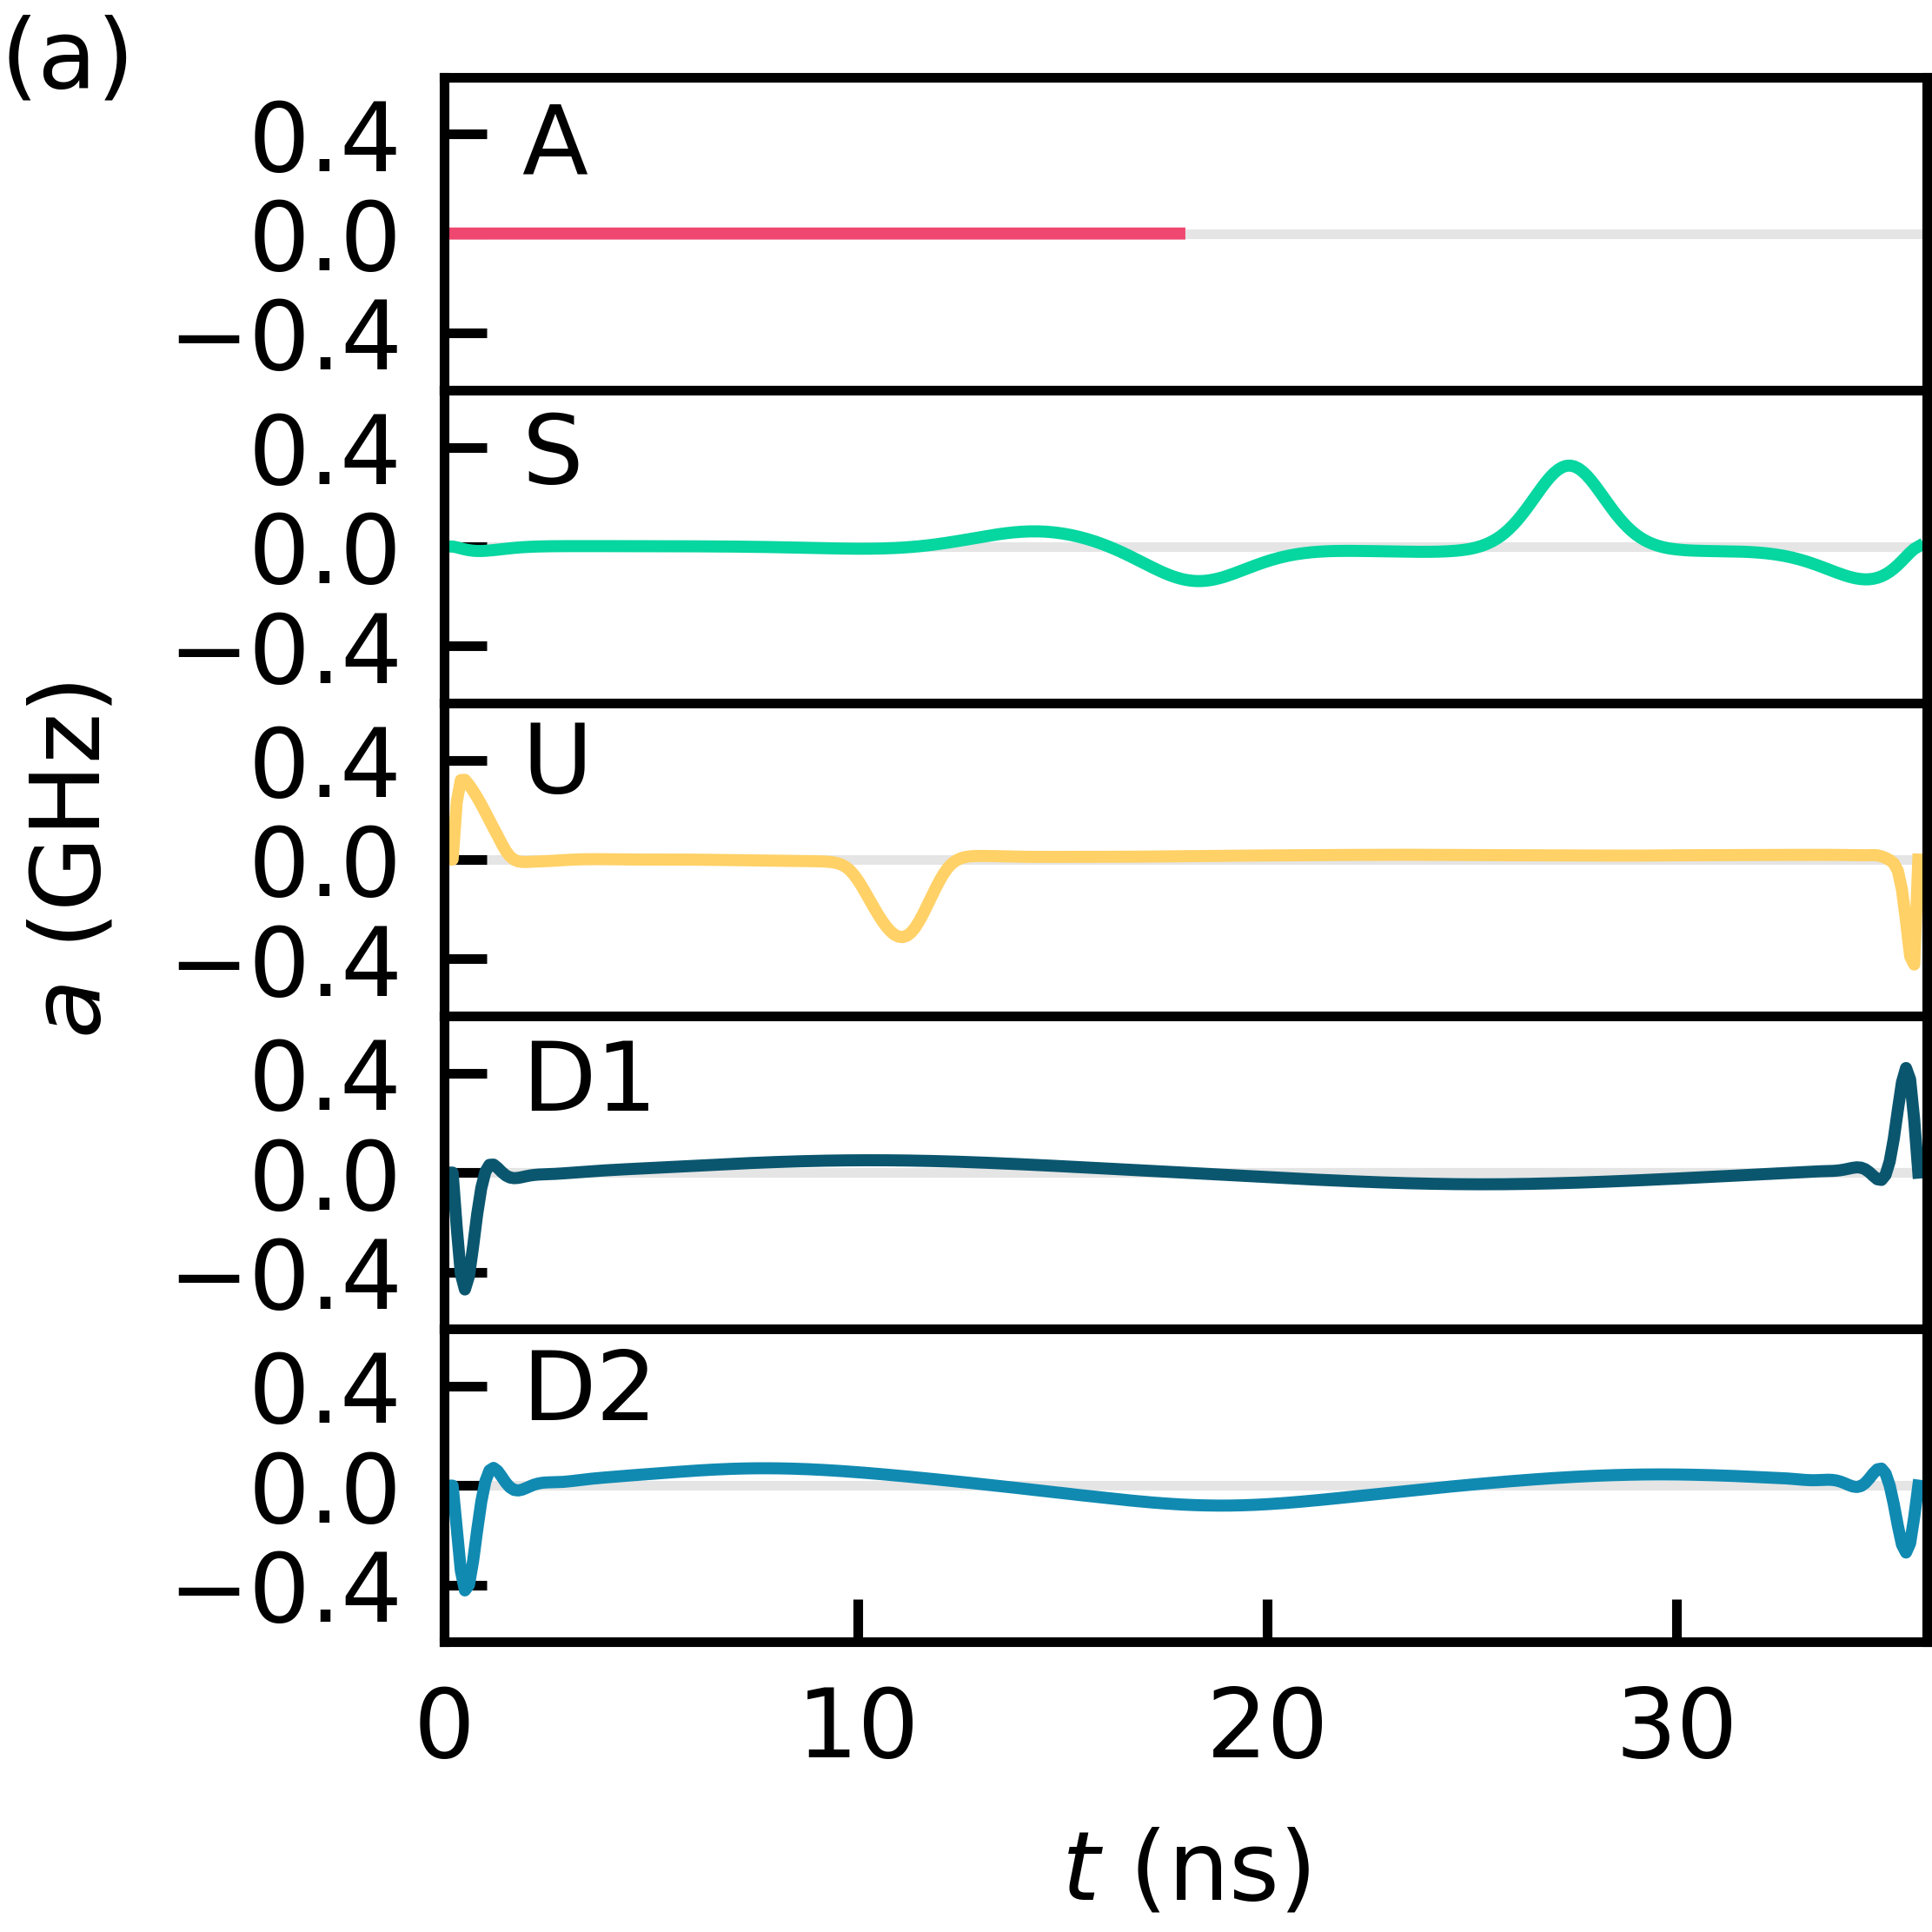
\includegraphics[width=\linewidth]{assets/f2a.png}
    \label{fig:statica}
  \end{subfigure}\hfill
  \begin{subfigure}{.4\textwidth}
    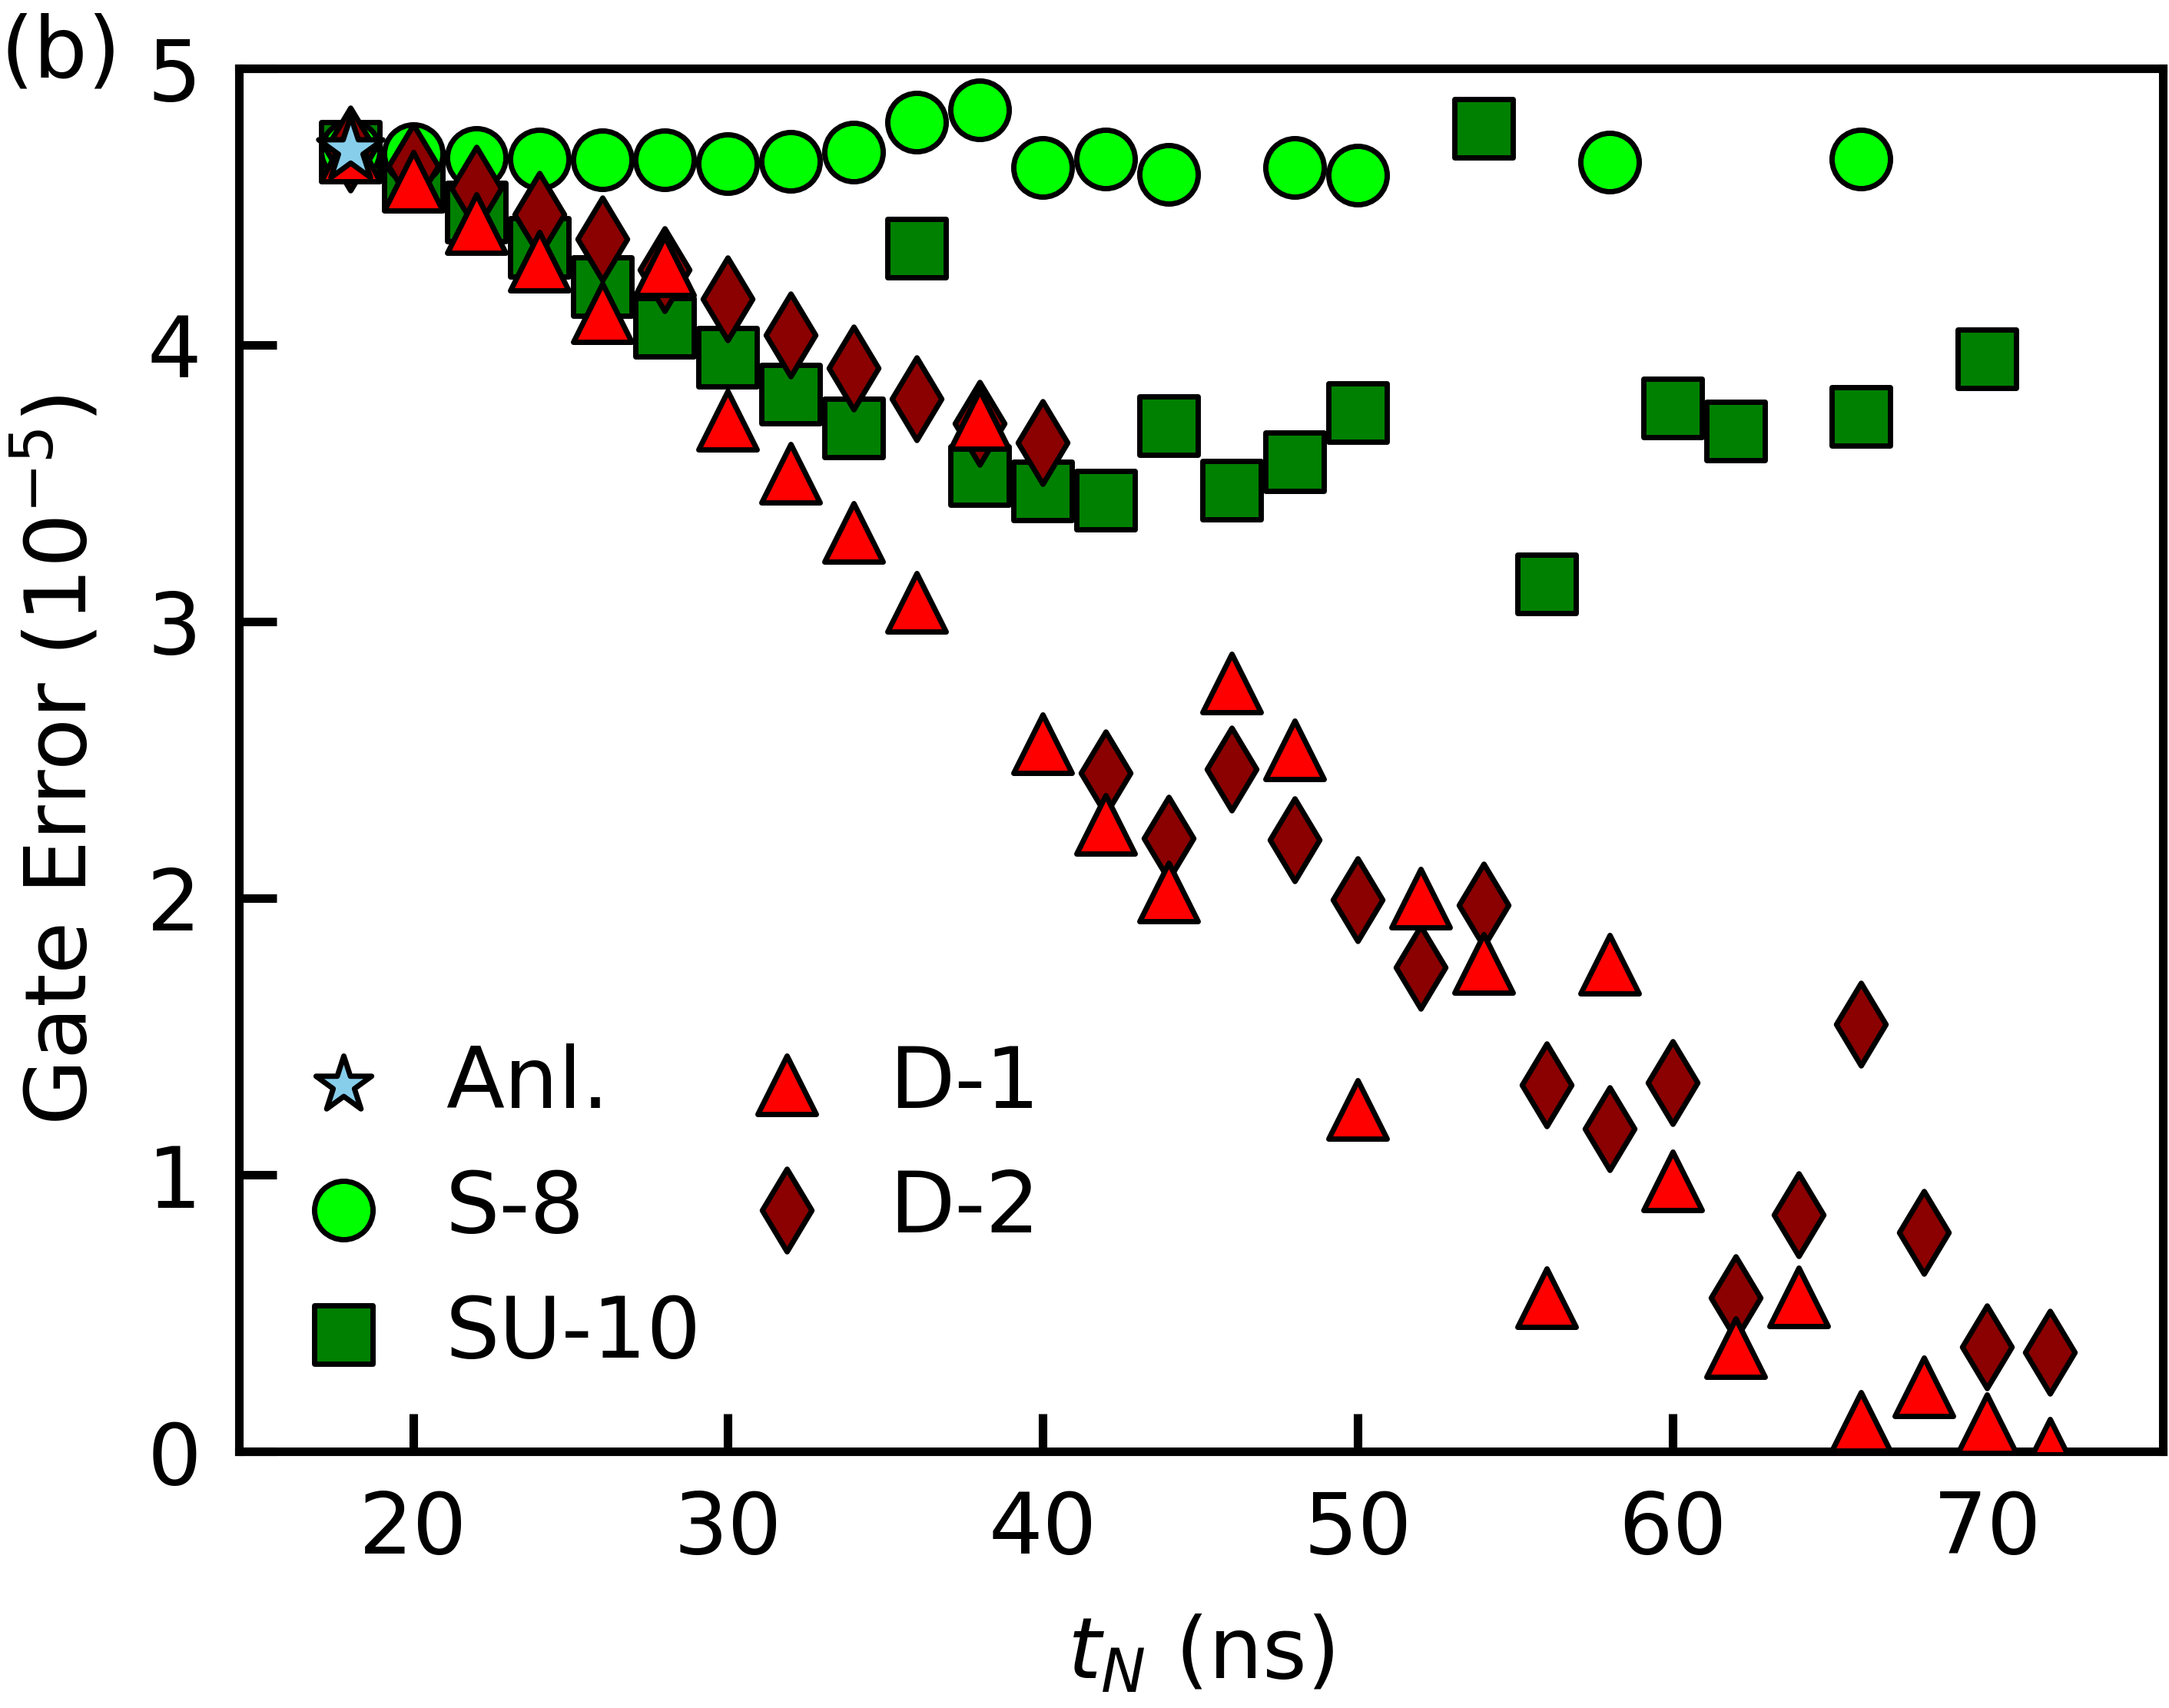
\includegraphics[width=\linewidth]{assets/f2c.png}
    \label{fig:staticb}
  \end{subfigure}\hfill
  \begin{subfigure}{.23\textwidth}
    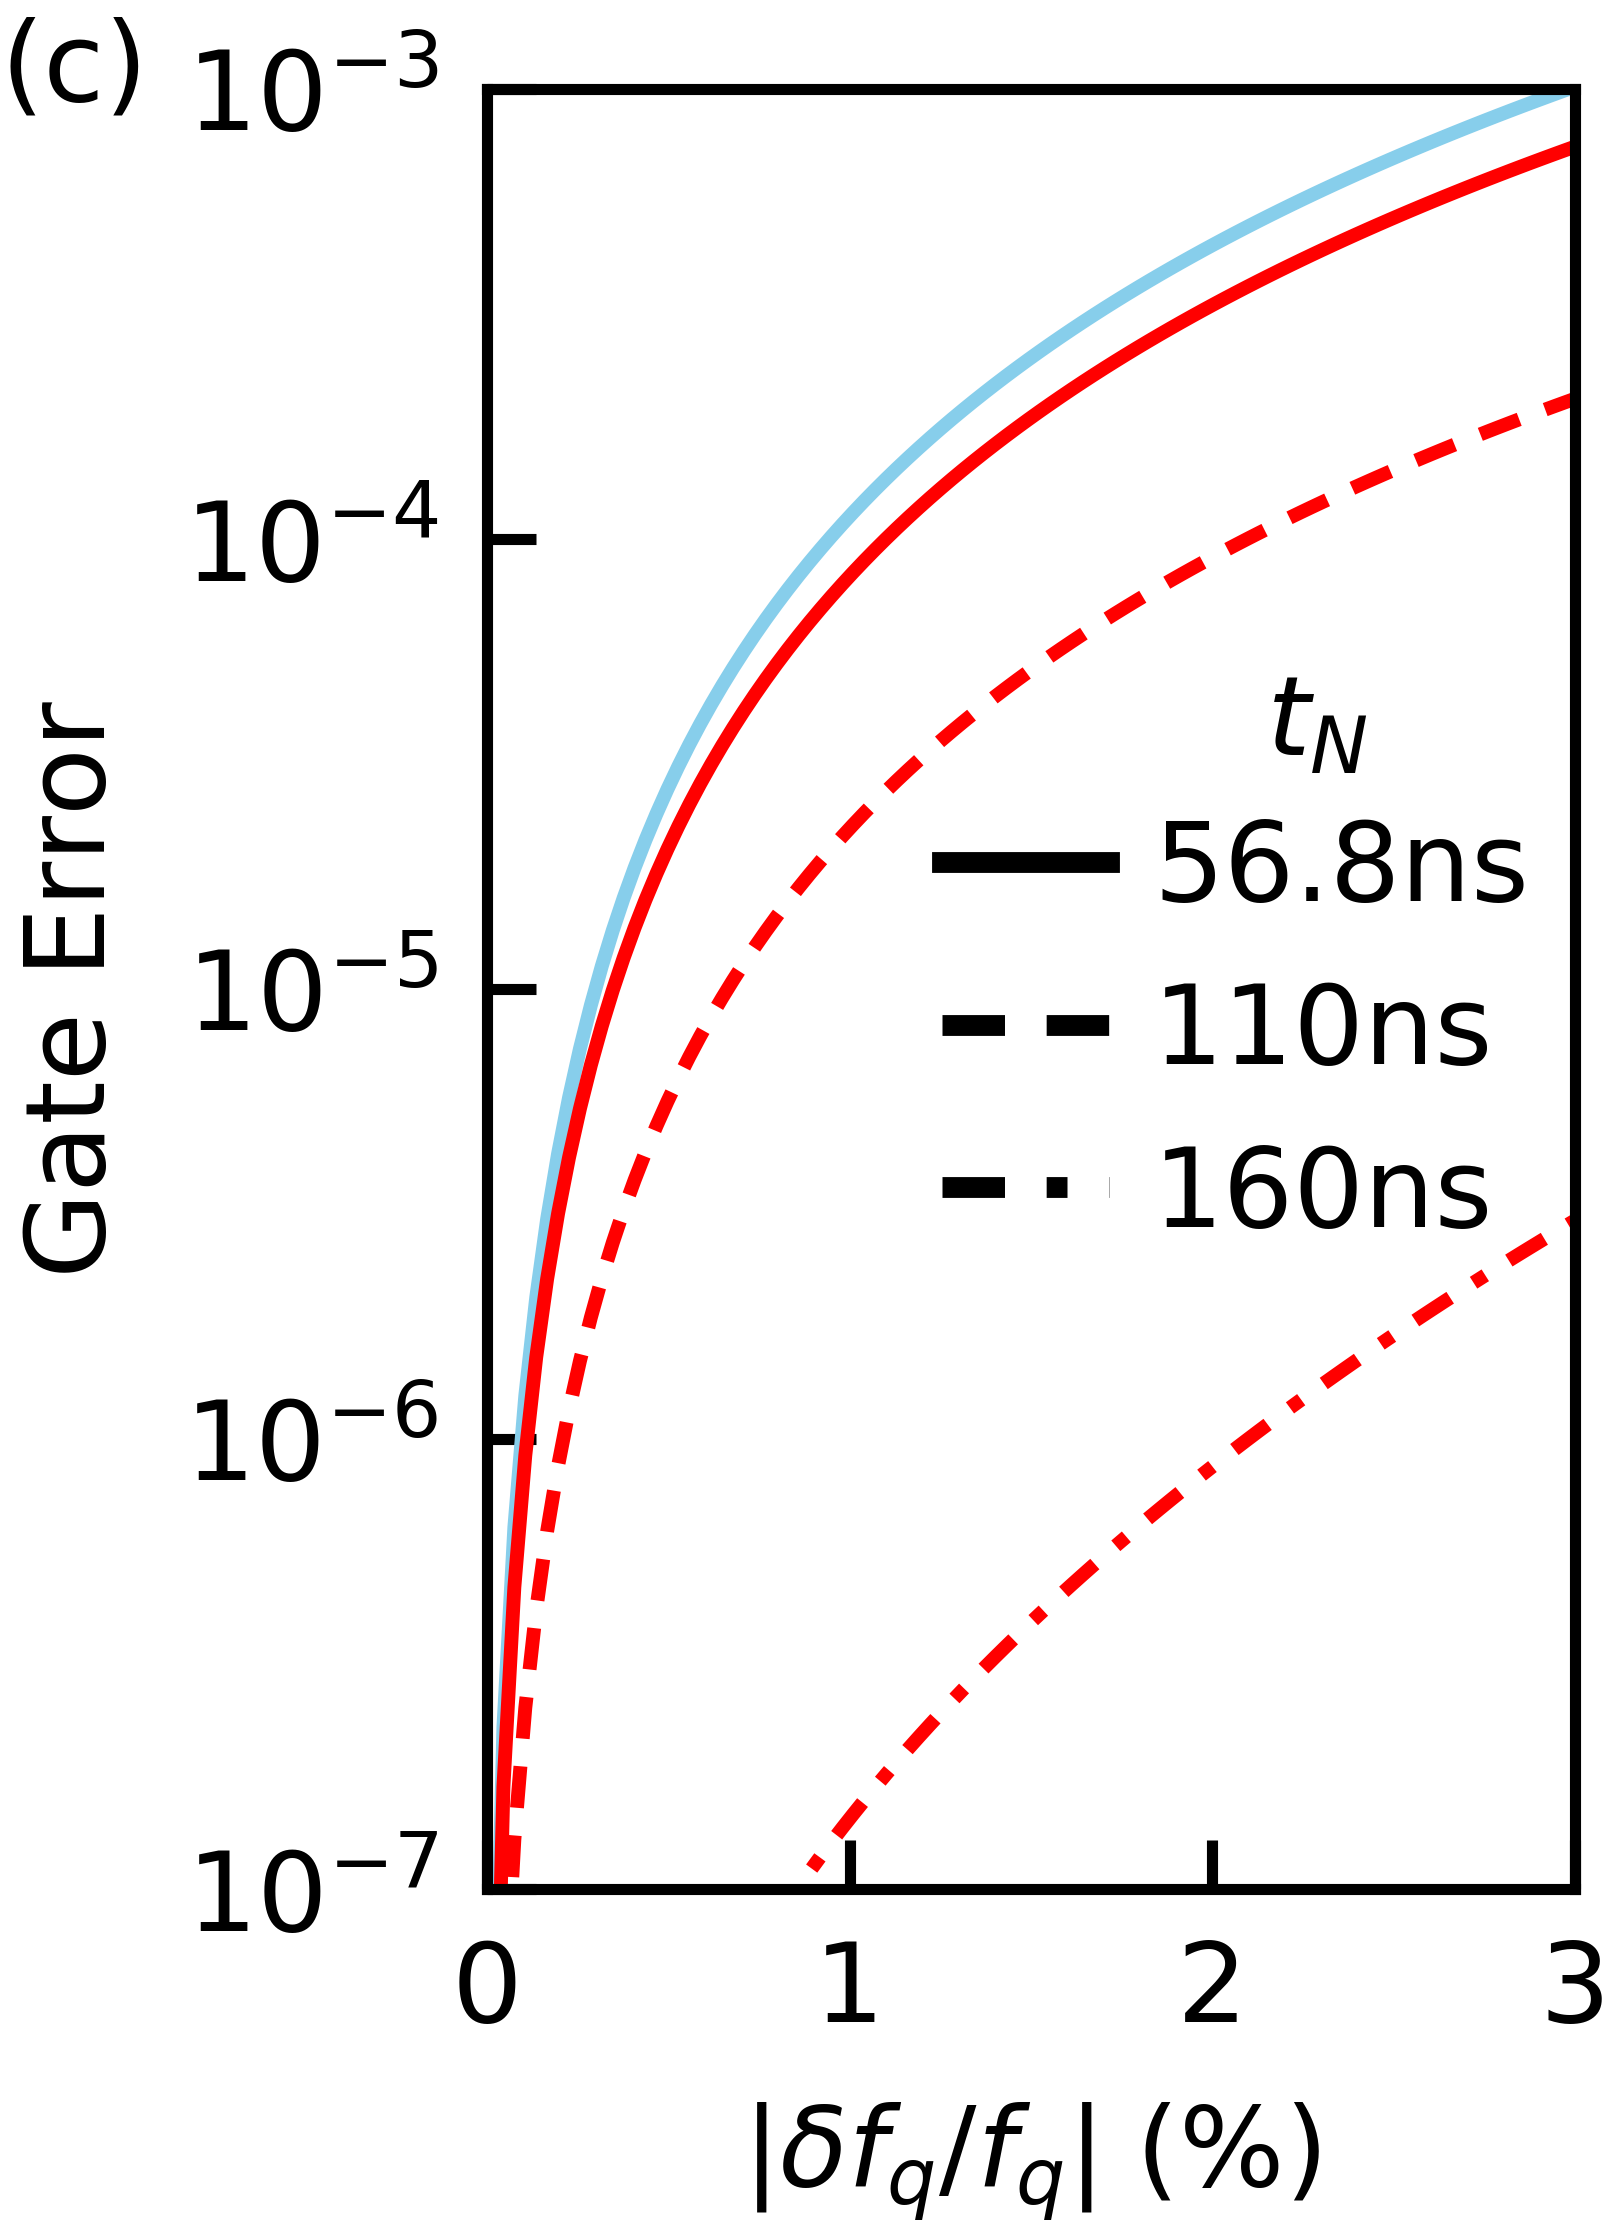
\includegraphics[width=\linewidth]{assets/f2b.png}
    \label{fig:staticc}
  \end{subfigure}
  \caption{
    (a) $Z/2$ gates robust to qubit frequency detunings constructed with the
    analytic, sampling, unscented sampling, and the 1\textsuperscript{st}-
    and 2\textsuperscript{nd}-order derivative methods. The gates
    shown for the numerical methods are the solutions at twice the analytic
    gate time.
    (b) Single gate error as
    a function of the gate duration at a one-percent
    detuning from the nominal qubit frequency for all methods. Missing
    data points represent solutions with a gate error above $5 \cdot 10^{-5}$.
    (c) Single gate error as a function of the detuning from the nominal
    qubit frequency. The solutions for the analytic and
    1\textsuperscript{st}-order derivative methods are shown at multiples
    of the analytic gate time. The performance of the two methods is
    indistinguishable at the analytic gate time $18$ns.
  }
  \label{fig:static}
\end{figure*}

We compare the numerical method we have developed to the analytic gates
on the task of achieving low gate errors in the presence of longitudinal relaxation
for the $Z/2$, $Y/2$, and $X/2$ gates.
The numerically optimized gates converge on similar solutions, a periodic
waveform with amplitude $\sim 0.2 \textrm{GHz}$, see Figure \ref{fig:longitudea}.
They extend their gate times
beyond their analytic counterparts, trading longer gate times for access
to higher amplitudes and therefore higher $T_{1}$ times. All numerical gates reduce
their single gate errors by a factor of $5$ over
their analytic counterparts which is commensurate to their
probability of longitudinal relaxation reductions, see Appendix \ref{appendix:longitude}.
The gate error reported in this text is the infidelity
of the evolved state and the target state averaged over 1000 pseudo-randomly
generated initial states. The numerical $Z/2$ and $Y/2$ gates perform simlarly in
the concatenated gate application comparision, suppressing cumulative gate errors to $8 \cdot 10^{-3}$
over $2000$ gate applications $\sim 40 \mu\textrm{s}$, see Figure \ref{fig:longitudec}.
The numerical $X/2$ gate achieves a cumulative gate error of
$1.7 \cdot 10^{-2}$ over $2000$ gate applications $\sim 124 \mu\textrm{s}$.
These low cumulative gate errors for high gate counts are critical for
noisy, intermediate-scale quantum (NISQ) applications.
Both the analytic and numerical gates attain single gate errors sufficient for
quantum error correction ($< 10^{-4}$), which are required for fault-tolerant quantum computing
\cite{aharonov2008fault, fowler2009high, gottesman1997stabilizer}.
These improvements are significant for the realistic constraints we have imposed
on the gates, and do not represent a fundamental limit to the optimization methods we have
employed.

